% --------------------- VARIABLEN -------------------------

\newcommand{\COURSE}{Physik und Materialwissenschaften\\ Praktikum Physik \\}
\newcommand{\SEMESTER}{Elektro- und Informationstechnik II}
\newcommand{\STUDENT}{Maximilian Spahn\\ und\\Benjamin Langer}

\newcommand{\HEADDING}{Praktikum Physik}
\newcommand{\SUBHEADDING}{Versuch 3.1: Spezifischer Widerstand und Halleffekt}

% ------------------- DEFINITIONEN -----------------------

\documentclass[a4paper]{scrartcl}

\usepackage[utf8]{inputenc}
\usepackage[ngerman]{babel}
\usepackage{amsmath}
\usepackage{amssymb}
\usepackage{color}
\usepackage{tikz}
\usepackage{float}
\usetikzlibrary{arrows,decorations.markings}
\usepackage{tabularx}
\usepackage{fancybox}
\usepackage{pgfplots}
\usepackage[colorlinks=false,linkcolor=black,urlcolor=blue,bookmarks,bookmarksopen=true]{hyperref}
\usepackage{geometry}
\usepackage{fancyhdr}

\usepackage[page]{totalcount}

%Größe der Ränder setzen
\geometry{a4paper,left=2cm, right=2cm, top=3cm, bottom=2cm, headheight=8cm}

%Kopf- und Fußzeile
\pagestyle {fancy}
\fancyhf{}
\fancyhead[L]{\STUDENT}
\fancyhead[C]{\COURSE}
\fancyhead[R]{\today}

\fancyfoot[L]{\SEMESTER}
\fancyfoot[C]{}
\fancyfoot[R]{Seite \thepage /\pageref{LastPage}}

%Formatierung der Überschrift, hier nichts ändern
\def\header#1#2{
  \begin{center}
    {\Large #1}\\
    {#2}
  \end{center}
}

\numberwithin{equation}{subsection}

\nocite{*}
\bibliographystyle{plain}

\setlength\parindent{0pt}

% ----------------------- DOCUMENT ---------------------------

\begin{document}

\vspace{10pt}
\header{\HEADDING}{\SUBHEADDING}

\tableofcontents

\newpage

\section{Einleitung}
Die Beiden Versuche, welche in dieser Ausarbeitung behandelt werden, beschäftigen sich mit den elektrischen Eigenschaften von Halbleitern. Im ersten behandeten Versuch wird dazu das Verhalten von Halbleitern anhand des Hall-Effekts veranschaulicht, also wie Elektronen in dem Halbleiter sich mit einer bestimmten Geschwindigkeit (Driftgeschwindigkeit) bewegen und somit auch durch die Lorenzkraft abgelenkt werden können. In der Theorie wird hierbei zusätzlich auch die Funktionsweise von elektrischen Leitern bis hin zu Halbleitern erklärt.
Ebenso wird in diesem Zusammenhang die Messung des spezifischen Widerstandes beleuchtet.

%TODO Hier kommt die Einleitung für den Zweiten Versuch 

\newpage

\section{Theorie}
\subsection{Leitfähigkeit von Materialien}
Der elektrische Strom wird durch die Bewegung von Ladungsträgern durch einen Leiter definiert.
Somit ergibt sich die Leitfähigkeit $\kappa$ eines Materials aus der Menge der verfügbaren, freien Ladungsträger $n$, deren Ladung $e$ und deren Beweglichkeit $\mu$. \cite{horn}

\begin{align}
\kappa = n \cdot e \cdot \mu
\end{align}

\subsubsection{Driftgeschwindigkeit}
Als Beweglichkeit ist die Geschwindigkeit des Ladungsträgers definiert. Wenn sich die Elektronen durch den Leiter bewegen, stoßen diese permanent mit den Atomrümpfen zusammen und werden so ausgebremst. Die mittlere Geschwindigkeit, also die Driftgeschwindigkeit ist für den spezifischen Widerstand mit verantwortlich. \cite{werk}

\subsubsection{Der  Elektrische Widerstand}
Der elektrische Widerstand ergibt sich aus dem Kehrwert der Leitfähigkeit also $\rho = \frac{1}{\kappa}$ geteilt durch die Fläche $A$ und mal die Länge $l$.
Wird die Querschnittsfläche des Leiters größer, kann sich der Storm sich mehr verteilen und der Widerstand wird kleiner. \cite{werk}

\begin{align}
R = \rho \frac{l}{A}
\end{align}

\subsubsection{Leitungsbänder}
Ein weiterer Faktor für die Leitfähigkeit ist die Anzahl, der freien Ladungsträger. Die Menge dieser lässt sich anhand der Orbitaltheorie begründen.
Die Elektronen sind um Atome in Atomorbitalen angeordnet. Dabei beschreiben Atomorbitale, Orte um den Atomrumpf, in welchem sich Elektronen aufhalten dürfen. Durch das Überlappen einer großen Anzahl an Atomorbitalen in Bindungen entstehen Bänder. (Abbildung~\ref{fig:orbital-bänder}) 
Bänder beschreiben kontinuierliche Zustände, in welchen sich die Elektronen aufhalten können. \\
Das Valenzband ist das höchste vollbesetzte Elektronen-Energieband (diese Elektronen sind für die Bindung der Atomrümpfe zuständig). Das Leitungsband ist das nächst höher gelegene Band. (Abbildung~\ref{fig:energiebänder})
Damit ein Elektron ein freier Ladungsträger wird, muss es seinen Platz in der Bindung verlassen und in ein unbesetztes Leitungsband springen. \cite{werk}

\begin{figure}[H]
\includegraphics[width=7cm]{Energiebänder}
\centering
\caption{Entstehung von Energiebänder \cite{tipler}}
\centering
\label{fig:orbital-bänder}
\end{figure}

\begin{figure}[H]
\includegraphics[width=2cm]{Energiebänder2}
\centering
\caption{Anordnung der Energiebänder \cite{werk}}
\centering
\label{fig:energiebänder}
\end{figure}

Bei metallischen Leiter, ist das Leitungsband teilweise gefüllt oder grenzt direkt an das Valenzband, somit ist zur Bewegung der Elektronen eine sehr geringe Energie nötig. Somit begründet sich auch die gute elektrische Leitfähigkeit von Metallen, da diese viele freie Ladungsträger haben. (Abbildung~\ref{fig:bandstrukturen_leiter-isolator}) \\

Bei Isolatoren dagegen ist eine große Energiedifferenz zu dem unbesetztes Leitungsband (Bandlücke), sodass diese keine freien Ladungsträger haben können.

\begin{figure}[H]
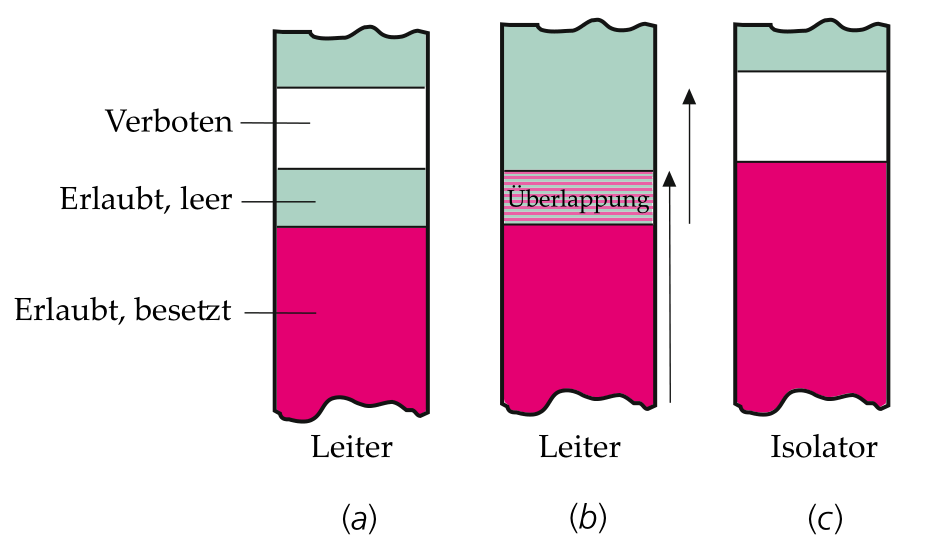
\includegraphics[width=10cm]{Bandstrukturen}
\centering
\caption{Bandstrukturen von Festkörpern. a: Ein typischer Leiter: Das Valenzband ist gleichzeitig das Leitungsband. b: Ein Leiter, bei dem das Valenzband das darüberliegende Leitungsband überlappt. c: Ein typischer Isolator: Das gefüllte Valenzband ist durch eine breite Bandlücke vom Leitungsband getrennt. \cite{tipler}}
\centering
\label{fig:bandstrukturen_leiter-isolator}
\end{figure}

\subsection{Halbleiter}
Halbleiter haben eine eher große Bandlücke, die das Valenzband von dem Leitungsband trennt.
Die Elektronen benötigen also eine bestimme Energie um die Bindung zu verlassen und als freie Ladungsträger zu agieren. \cite{werk}
Die fehlenden Elektronen im Valenzband werden Defektelektronen oder Löcher genannt. Sie verhalten sich wie positive Teilchen. \cite{hering}
Sowohl die Bewegung des freien Elektrons sowie die Bewegung des Lochs tragen zur Leitfähigkeit bei.

\subsubsection{Dotierung}
Um die nötige Energie, die die Elektronen benötigen zu verringern, werden Halbleiter dotiert. Dabei werden andere Atome mit mehr oder weniger Valenzelektronen als das Wirtsgitter in den Halbleiter eingebracht. 
Die zusätzlichen Elektronen lassen sich leichter lösen als die Bildungselektronen und die "fehlenden" Elektronen begünstigen die Entstehung von Löchern. Dies liegt daran, dass das bei der n-Dotierung das Donatorniveau durch die zusätzlichen Elektronen näher am Leitungsband liegt und Elektonen weniger Energie brauchen, um in den freien Zustand zu gelangen. \cite{werk}

\begin{figure}[H]
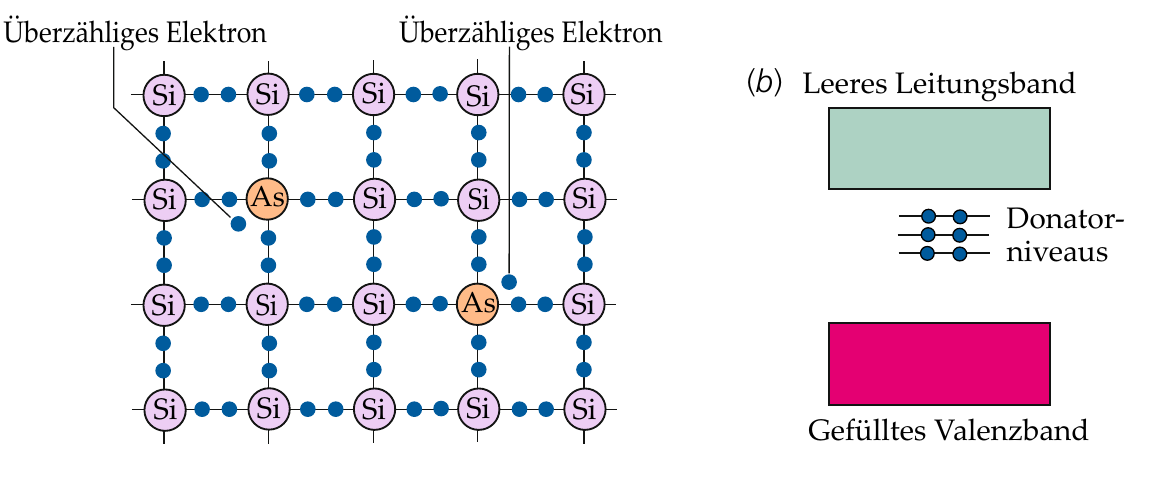
\includegraphics[width=12cm]{n-dotierter_Halbleiter}
\centering
\caption{Bandstruktur eines n-Dotierten Halbleiters \cite{tipler}}
\centering
\label{fig:bandstruktur-n-dotiert}
\end{figure}

Genauso liegt bei der p-Dotierung das Akzeptorniveau aufgrund des fehlendes Valenzelektron näher am Valenzband, wodurch auch hier weniger Energie für die Entstehung von Löchern benötigt wird. \cite{werk}

\begin{figure}[H]
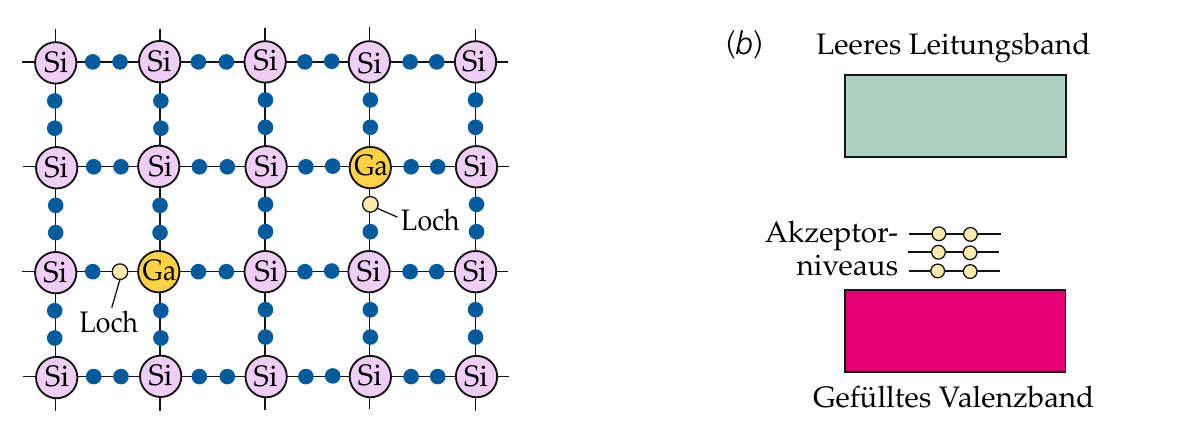
\includegraphics[width=12cm]{p-dotierter_Halbleiter}
\centering
\caption{Bandstruktur eines p-Dotierten Halbleiters \cite{tipler}}
\centering
\label{fig:bandstruktur-p-dotiert}
\end{figure}

\subsubsection{pn-Übergang}
%TODO hier kommt die Erklärung zum pn-Übergang und was sonst so noch allgemein für Halbleiter erklärt werden muss

\subsection{Messung Spezifischer Widerstand nach van der Pauw}
Mit dem Verfahren nach van der Pauw kann der Flächenwiderstand $R_{\square}$ einer dünnen, planparallelen Platte fast beliebiger Form zu bestimmt werden. Der Flächenwiderstand einer dünnen, planparallelen Platte der Dicke $d$ ist der spezifische Widerstand $\rho$ dividiert durch die Dicke der Platte. 

\begin{align}
R_{\square} = \frac{\rho}{d}
\end{align}

Somit lässt sich das Verfahren nutzen um den Spezifischen Widerstand eines Materials beliebiger Form zu messen. \cite{anl}
Das Verfahren wird gegenüber der Vierspitzenmessmethode Messmethode bevorzugt, da es den spezifischen Widerstand eine 2D-Fläche und nicht in eine lineare Richtung misst. \cite{phyglob} \\

Zur Durchführung der Messung werden vier sehr kleine Kontakte am äußeren Rand der zu messenden Probe angebracht (Abbildung 1). Die Probe muss hierbei auf ihrer gesamten Fläche die gleiche Dicke d haben und darf keine Löcher bzw. isolierte Bereiche in ihrem Inneren aufweisen. \cite{anl} \\

Anschließend wird über die Kontakte A und B ein konstanter Strom I eingeprägt und die Spannung über C und D gemessen. Daraus berechnet sich der charakteristische Widerstand: \cite{phyglob}

\begin{align}
R_{AB,DC} = \frac{U_{DC}}{I_{AB}}
\end{align}

Darauf wird dementsprechend in Strom über die Kontakte B und C eingeprägt und die Spannung über A und D gemessen. Darus ergibt sich der Widerstand $R_{BC,AD}$ \cite{anl} \\

Mit den Beiden Widerständen lässt sich anschließend nach van der Pauw der Flächenwiderstand berechnen. \cite{anl}

\begin{align}
R_{\square} = \frac{\pi}{ln(2)} \cdot \frac{(R_{AB,DC}+R_{BC,AD})}{2} \cdot f(x)
\end{align}

Dabei ist $f(x)$ der Geometriefaktor (Korrekturfaktor) der entsprechend der Quelle \cite{anl} vereinfacht wie folgt berechnet wird. Dabei sind $x$ und $z$ Hilfsgrößen zur Berechnung.

\begin{align}
x = \frac{R_{AB,DC}}{R_{BC,AD}}
\end{align}

\begin{align}
z = \frac{ln(2)}{2} \cdot \left(\frac{x-1}{x+1}\right)^2
\end{align}

\begin{align}
f(x) = 1 - z - \left( 1-\frac{ln(2)}{3}\right)  \cdot z^2 - \left( 2 - \frac{4}{3} \cdot ln(2) + \frac{8}{45} \cdot ln^2(2)\right) \cdot z^2
\end{align}

\subsection{Halleffekt}
Der Halleffekt basiert grundsätzlich auf der Lorenzkraft, welche auf die Elektronen in einem, im Magnetfeld befindlichen, Halbleiter wirkt.

\subsubsection{Lorentzkraft}
Ladungsträger, die sich mit einer Geschwindigkeit $\overrightarrow{v}$ durch ein Magnetfeld $\overrightarrow{B}$ bewegen, werden durch die Lorentzkraft abgelenkt. 
Die Richtung der Lorentzkraft $\overrightarrow{F_L}$ hängt von der Ladung der Ladungsträger $q$, deren Bewegungsrichtung $\overrightarrow{v}$ und der Richtung des Magnetfeldes bzw. der Flussdichte $\overrightarrow{B}$ ab. \cite{anl}

\begin{align}
\overrightarrow{F_L} = q \cdot (\overrightarrow{v} \times \overrightarrow{B})
\end{align}

\subsubsection{Berechnung der Hall-Spannung}

Durch die Ablenkung der Elektronen im Magnetfeld entsteht auf der linken Seite des Halbleiters ein Überschuss an Elektronen, sie lädt sich negativ auf. Auf der Gegenseite verbleibt die positive Ladung der ortsfesten Donatoren. Durch die Ladungsdifferenz entsteht in dem Leiter ein elektrisches Feld. Dieses Feld lässt eine entgegengesetzte Kraft $\overrightarrow{F_H}$ auf die Elektronen wirken. Durch das Gleichsetzen dieser beiden Kräfte, lässt sich die Stärke des Feldes, bzw. die Hallspannung $U_H$ berechnen. \cite{anl}

\begin{align}
\overrightarrow{F_H} &= -\overrightarrow{F_L} \\
\overrightarrow{E_H} \cdot q &= -(q \cdot (\overrightarrow{v} \times \overrightarrow{B})) \\
\frac{U_H}{b} &= v \cdot B \text{(für $v \perp B$)}
\end{align}

\begin{align}
\Rightarrow U_H = v \cdot B \cdot b
\end{align}

Die Drittgeschwindigkeit der Elektronen, welche ausschlaggebend für die Lorenzkraft ist, ergibt sich aus der Stromdichte in dem Halbleiter. \cite{anl}

\begin{align}
j = \frac{I}{b \cdot d} und j = n \cdot q \cdot v
\end{align}

\begin{align}
\Rightarrow v = \frac{I}{n \cdot q \cdot b \cdot d}
\end{align}

Die Beiden Gleichungen ineinander eingesetzt ergibt als Hallspannung:

\begin{align}
U_H = \frac{1}{n \cdot q} \cdot \frac{I \cdot B}{d}
\end{align}

Dabei ist der Faktor $A_H = \frac{1}{n \cdot q}$, auch Hall-Koeffizient welcher auch über die Art der Ladungsträger aussagt. Der Hall-Koeffizient ist positiv für Löcherleitung $(q = +e)$ und negativ für Elektronenleitung $(q = -e)$. \cite{anl}

\subsubsection{Messung der Hallspannung}

Bei der Messung der Messung der Hallspannung muss bedacht werden, dass keine Probe perfekt symmetrisch ist und somit auch eine Querspannung anliegt, auch ohne das Vorhandensein eines äußeren Magnetfeldes. Die Hallspannung UH ist die Differenz zwischen Querspannung mit und ohne Magnetfeld. \cite{anl}

\begin{align}
U_H = U_{BD,\text{mit}} - U_{BD,\text{ohne}}
\end{align}

\subsection{Was auch immer für Versuch 2 an Theorie ist}

%TODO

\newpage

\section{Versuch 3.1 Spezifischer Widerstand und Halleffekt}
\subsection{Häusliche Vorarbeit}
\subsubsection{3.3.2 - Van der Pauw Widerstandsnetzwerk}
Die Probe besteht aus einer Art Gitter aus widerständen. Dabei ist jeder Punkt der Probe nach links, rechts, oben, unten mit einem benachbarten Punkt über einen Widerstand vernetzt. Dabei kann man sich einen Widerstand im Netzwerk ersatzweise als spezifischen Widerstand des Materials vorstellen vorstellen. Nach folgendem Aufbau verteilt sich der Strom auf die verschiedenen Widerstände. Dabei fließt durch die Widerstände auf der direkten Strecke zwischen VCC und GND der Hauptanteil des Stromes und je weiter man nach rechts kommt immer weniger. Dennoch wird auch an den äußeren Widerständen zwischen B und C ein messbarer Spannungsabfall erzeugt.

\begin{figure}[H]
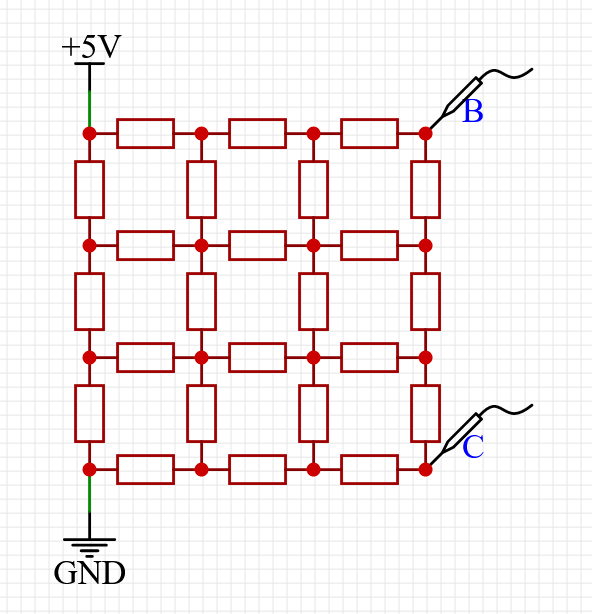
\includegraphics[width=7cm]{Widerstandsnetzwerk_v3}
\centering
\caption{Widerstandsnetzwerk bei der van der Pauw Messung}
\centering
\label{fig:widerstandsnetzwerk}
\end{figure}

Die folgende Grafik zeigt die Stromdichteverteilung in dem Netzwerk dabei kann man an den eigezeichneten Potentiallinien erkennen, Welche spannung an B und C gemessen wird wenn der Strom von A nach D fließt

\begin{figure}[H]
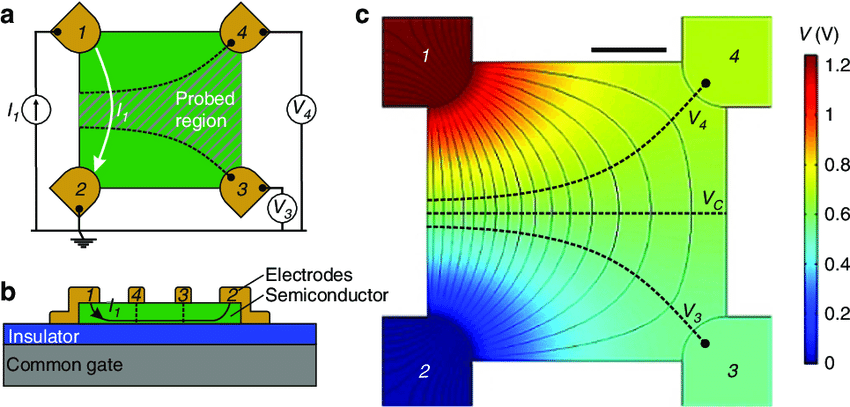
\includegraphics[width=12cm]{Top-view-of-van-der-Pauw-square-shaped}
\centering
\caption{Stromdichteverteilung bei der van der Pauw Messung \protect\footnotemark}
\centering
\label{fig:top-view-of-van-der-pauw}
\end{figure}

\footnotetext{\url{https://www.researchgate.net/figure/The-gated-van-der-Pauw-method-a-Top-view-of-a-van-der-Pauw-device-with-square-shaped_fig4_316052617}}

\subsubsection{3.3.3 - Zeichnung zum Halleffekt im p-Halbleiter}
Die folgende Abbildung zeigt alle Felder, Spannungen und Ströme für einen p-Halbleiter.

\begin{figure}[H]
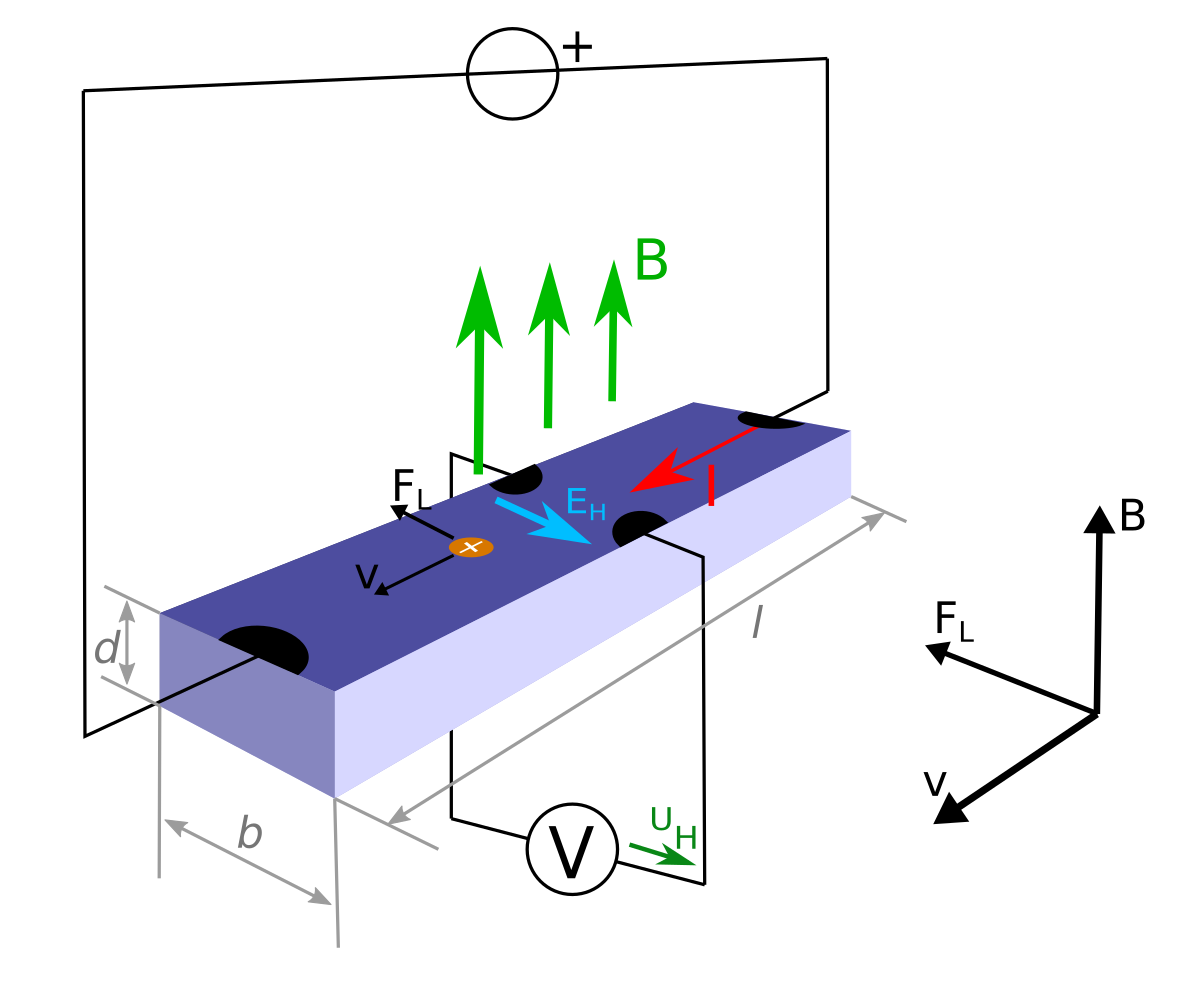
\includegraphics[width=12cm]{p-Halbleiter_Hall-Effekt}
\centering
\caption{Halleffekt im p-Halbleiter}
\centering
\label{fig:halleffekt-p-halbleiter}
\end{figure}

\subsubsection{3.3.4 - Ladungsträgerdichte von Silizium}
In den Beispielaufgaben zum der Ladungsträgerdichte von Silizium werden in dem Arbeitsbuch "Physik für Studierende der Naturwissenschaften und Technik" (vgl. \cite{tipler}) $5 \cdot 10^{16} \frac{\text{Elektronen}}{cm^3}$ als typische Werte angenommen. Dies stimmt auch mit dem in der folgenden Grafik (Abbildung~\ref{fig:spezifischer-widerstand-silizium}) markierten Bereich überein.

\subsubsection{3.3.5 - Abhängigkeit des spezifischer Widerstands von der Dotierung}
Die folgende Grafik (Abbildung~\ref{fig:spezifischer-widerstand-silizium}) zeigt die Abhängigkeit des spezifischer Widerstands in Silizium von der Dotierung. 
Dabei lässt sich ein größtenteils linearer Zusammenhang erkennen, wobei der widerstand eines p-Dotierten Halbleiters leicht größer ist.

\begin{figure}[H]
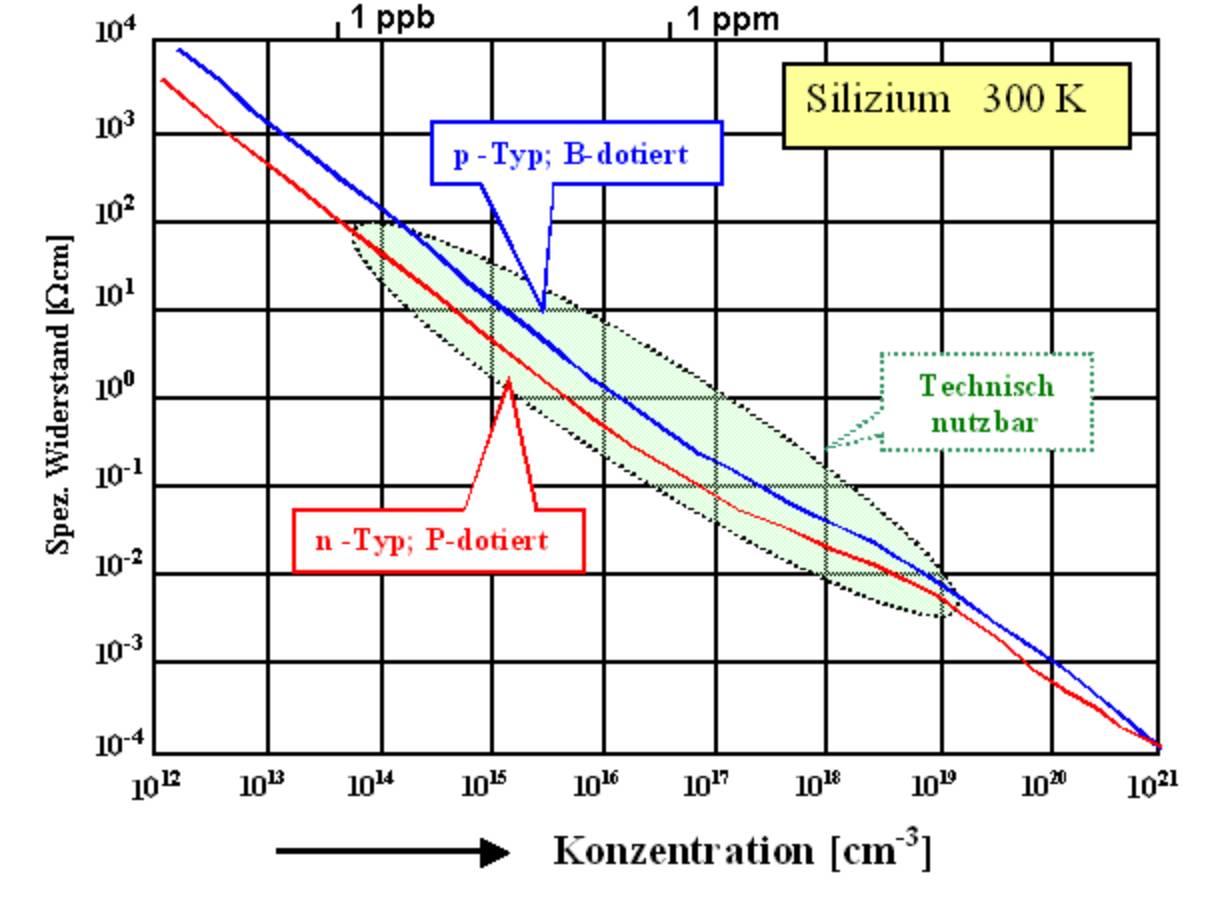
\includegraphics[width=12cm]{spezifischer_Widerstand_Silizium}
\centering
\caption{Abhängigkeit des spezifischer Widerstands von der Dotierung \protect\footnotemark}
\centering
\label{fig:spezifischer-widerstand-silizium}
\end{figure}

\footnotetext{\url{https://www.tf.uni-kiel.de/matwis/amat/mw2_ge/kap_5/backbone/r5_3_1.html}}

\subsubsection{3.3.6 - Abhängigkeit der Beweglichkeit der Elektronen / Löcher von der Dotierung}
Die folgende Abbildung zeigt die Beweglichkeit als Funktion der Elektronen–Konzentration in Ge, Si, GaAs bei Raumtemperatur. Dabei ist zu erkennen, dass die Beweglichkeit der Elektronen (in rosa) höher ist als die der Löcher (in hellblau)

\begin{figure}[H]
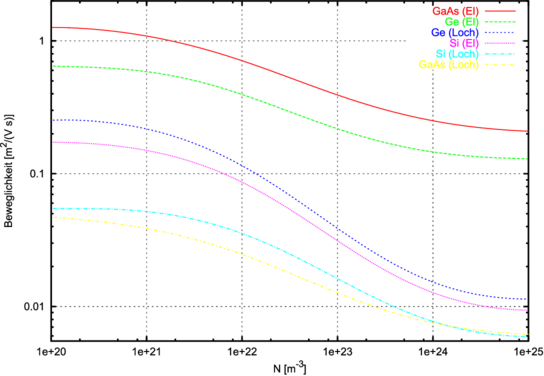
\includegraphics[width=12cm]{beweglichkeit-Silizium}
\centering
\caption{Beweglichkeit als Funktion der Elektronen–Konzentration in Ge, Si, GaAs bei Raumtemperatur \protect\footnotemark}
\centering
\label{fig:beweglichkeit-silizium}
\end{figure}

\footnotetext{\url{http://wwwex.physik.uni-ulm.de/lehre/physikalischeelektronik/phys_elektr/phys_elektrse10.html}}

\subsubsection{3.3.7 - Richtung des Magnetfelds eines Stabmagneten}
Die Folgende Grafik zeigt die Feldlinien eines Stabmagneten. Dabei gehen die Feldlinien senkrecht aus dem (roten) Nordpol hervor und gehen danach wider senkrecht in den Südpol (grün) herein.

\begin{figure}[H]
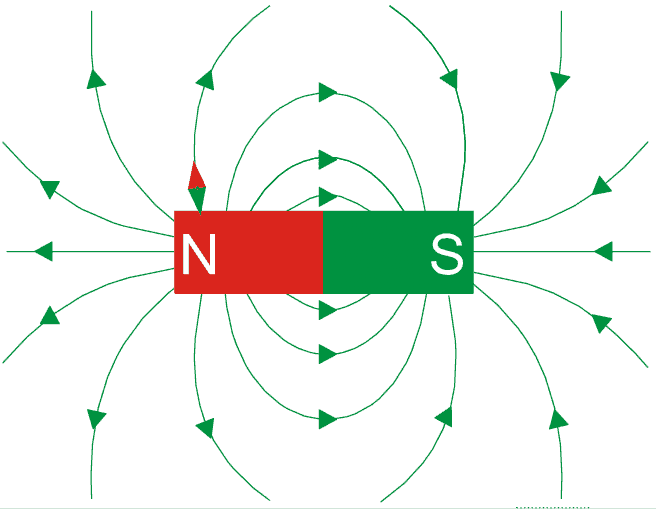
\includegraphics[width=8cm]{stabmagnet}
\centering
\caption{Magnetfelds eines Stabmagneten \protect\footnotemark}
\centering
\label{fig:stabmagnet}
\end{figure}

\footnotetext{\url{https://www.leifiphysik.de/elektrizitaetslehre/permanentmagnetismus/grundwissen/magnetfeld-und-feldlinien}}

\subsubsection{3.3.8 - }

\newpage

\subsection{Aufbau und Durchführung}
\subsubsection{Teil A: Bestimmung des spezifischen Widerstands}

Die Messschaltung wird wie in der folgenden Schaltung aufgebaut. (Abbildung~\ref{fig:messchaltung-spezifischer-widerstand})
Dazu wird der Probenhalter mit der Si-Prode (Abbildung~\ref{fig:probehalter-mit-si}) in die Messbox (Abbildung~\ref{fig:messbox-mit-anschluss}) eingebaut und die Messgeräte entsprechend des Schaltplanes angeschlossen.

\begin{figure}[H]
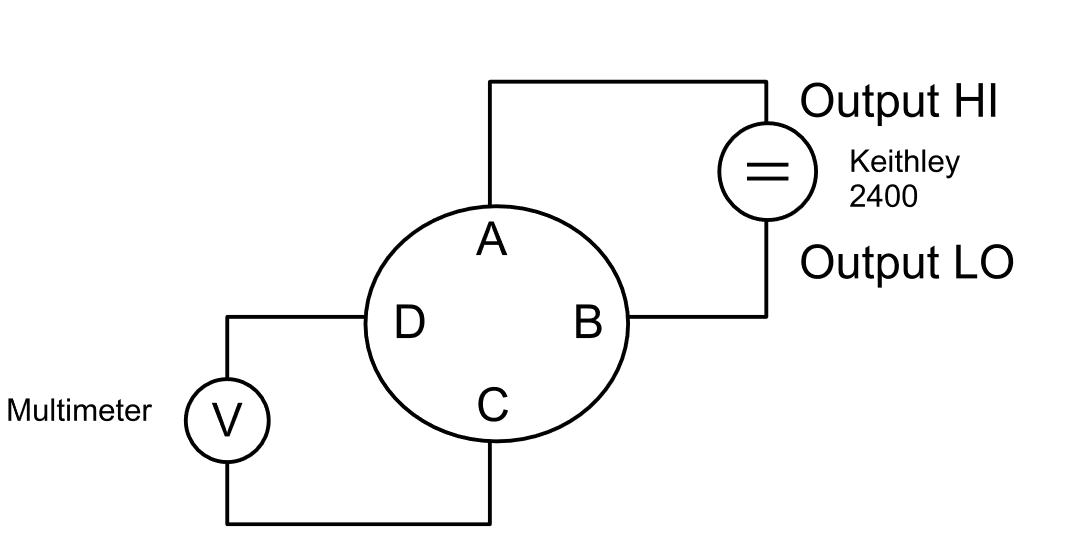
\includegraphics[width=12cm]{messchaltung_spezifischer_Widerstand}
\centering
\caption{Messschaltung zur Bestimmung des spezifischen Widerstandes \cite{anl}}
\centering
\label{fig:messchaltung-spezifischer-widerstand}
\end{figure}

\begin{figure}[H]
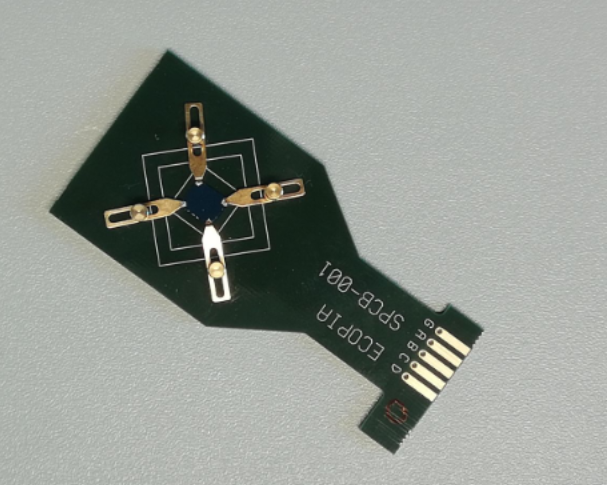
\includegraphics[width=7cm]{probehalter-mit-si}
\centering
\caption{Probenhalter mit montierter Si-Probe \cite{anl}}
\centering
\label{fig:probehalter-mit-si}
\end{figure}

\begin{figure}[H]
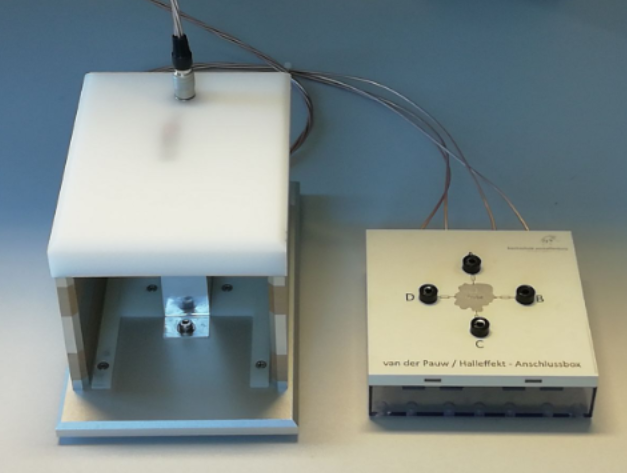
\includegraphics[width=7cm]{messbox_mit_anschluss}
\centering
\caption{Messbox mit Anschlussbox \cite{anl}}
\centering
\label{fig:messbox-mit-anschluss}
\end{figure}

Nun wird der Spezifische Widerstand wie bereits in dem Theorieteil beschrieben gemessen.
Dazu wird für Verschiedene Ströme (zuerst über A nach B dann über B nach C) die Spannung über D-C bzw. A-D gemessen
Mit der dicke der Probe lässt sich nun der spezifische Widerstand gemessen.

\subsubsection{Teil B: Bestimmung der Art der Ladungsträger}

Die Probe wird aus der Messbox entfernt und die Hallspannung wie in (Abbildung~\ref{fig:messchaltung-hall}) gemessen, während einmal der Nordpol und einmal der Südpol darüber gehalten wird. Eine Messung ohne Magnet erlaubt es den Drift (siehe Theorieteil) aus den Ergebnissen zu eliminieren.

\begin{figure}[H]
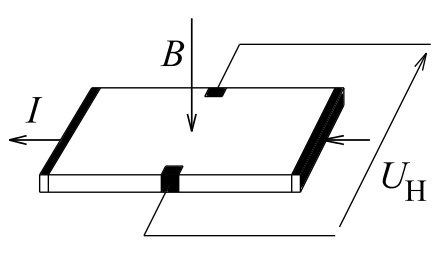
\includegraphics[width=8cm]{messchaltung_hall}
\centering
\caption{Messschaltung zur Bestimmung der Hall-Spannung \protect\footnotemark}
\centering
\label{fig:messchaltung-hall}
\end{figure}

\footnotetext{\url{https://de.wikipedia.org/wiki/Hall-Sensor}}

Die Messungen werden an einer p-Dotierten und einer n-Dotierten Germaniumprobe wiederholt und mit der Siliziumprobe, zu welcher die Dotierung unbekannt ist verglichen. Daraus lässt dich die Dotierung der Si-Probe bestimmen.

\subsubsection{Teil C: Bestimmung der Ladungsträgerdichte und Beweglichkeit}

Der Messadapter (weißer Kunststoffdeckel) mit eingebautem Probenhalter wieder vorsichtig in die Messbox eingebaut.
Anschließend wird die Hallspannung mit Dauermagnet (von forne und von hinten eingeschoben) gemessen.
Eine Messung ohne Magnet soll wider den Drift kompensieren.\\

Anschließend wird für beide Zustände des Magneten das Magnetfeld gemessen. \\

Aus den Messergebissen lässt sich die Ladungsträgerdichte und Beweglichkeit berechnen

\newpage

\subsection{Auswertung Versuch}

\newpage

\subsection{Wertung/Fazit}

\newpage


\section{Versuch 3.2 pn-Übergang... oder so... hab kein plan}
\subsection{Häusliche Vorarbeit}

\newpage

\subsection{Aufbau und Durchführung}

\newpage

\subsection{Auswertung Versuch}

\newpage

\subsection{Wertung/Fazit}

\newpage

\section{Brauchen wir einen Anhang für Tabellen?}

\newpage

\bibliography{literatur}




\label{LastPage}
\end{document}
%%% Local Variables:
%%% mode: latex
%%% TeX-master: t
%%% End: